\documentclass{article}
\usepackage{graphicx}
\usepackage{amsmath}
\title{A Closed Form for the Sum of the First $N$ Integers}
\author{A. Tester \\ Institute for Harness Demonstrations}
\date{2026}

\begin{document}
\maketitle

\begin{abstract}
We restate and numerically verify the classical identity
$\sum_{k=1}^{N} k = N(N+1)/2$. While elementary, the result serves as a
self-contained fixture for exercising automated publication tooling: it has a
manuscript, a single reproducible figure, and a one-line method.
\end{abstract}

\section{Introduction}
The triangular numbers $T_N = \sum_{k=1}^{N} k$ appear throughout
combinatorics. We give the closed form and verify it computationally.

\section{Method}
By pairing the first and last terms, the sum of the first $N$ positive
integers is
\begin{equation}
\label{eq:closed-form}
T_N = \sum_{k=1}^{N} k = \frac{N(N+1)}{2}.
\end{equation}

\section{Results}
Figure~\ref{fig:growth} compares the direct summation against the closed form
in Equation~\eqref{eq:closed-form} for $N = 1 \dots 100$; the two agree to
machine precision (maximum absolute difference $0$).

\begin{figure}[h]
\centering
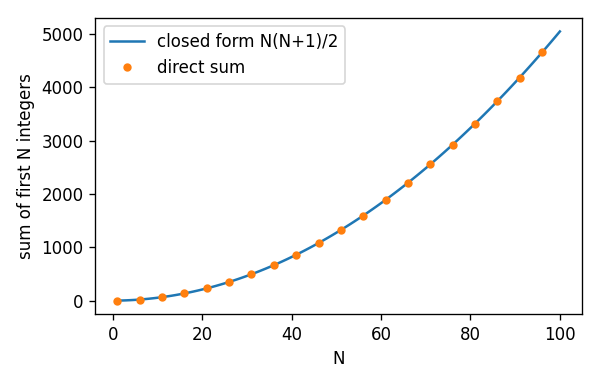
\includegraphics[width=0.7\linewidth]{figures/fig1.png}
\caption{Direct sum (points) versus the closed form (line). They coincide.}
\label{fig:growth}
\end{figure}

\section{Conclusion}
The closed form is exact. This paper exists to test agentic publication.

\end{document}
